\documentclass[12pt]{article}
\usepackage{multicol}
\usepackage[margin=0.4in]{geometry}
\include{pythonlisting}
\title{Graph Theory Note}
\usepackage{tikz}
\usetikzlibrary{automata, positioning, arrows}
\author{Ran Xie}

\begin{document}
	\twocolumn
	\maketitle
	\section{Regular Languages}

% { \epsilon }
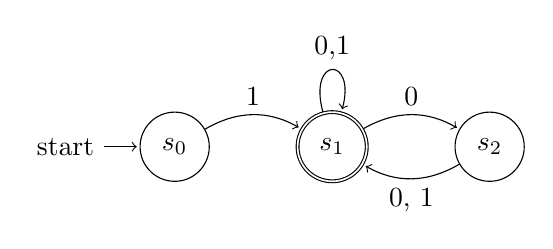
\begin{tikzpicture}[shorten >=1pt,node distance=2cm,on grid,auto]
	
	\node[state,initial]  (s_0)     {$s_0$};
	\node[state,accepting] (s_1) [right of=s_0]    {$s_1$};
	\node[state]  (s_2) [right of=s_1]  {$s_2$};
	
	\path[->]
	(s_0) edge [bend left]     node {1}  (s_1)
	(s_1) edge [loop above]  node {0,1}  ()
	      edge [bend left] node {0} (s_2)
	(s_2) edge [bend left] node {0, 1} (s_1);
\end{tikzpicture}

\textbf{state diagram} of \textbf{finite automaton} $M$. $q_0,q_1,q_2$ are \textbf{states}. $q_0$ is \textbf{start state}. $q_1$ is \textbf{accept state}. Arrows are called \textbf{transitions}. Input is string of 0s and 1s. The output is either \textbf{reject} or \textbf{accept}.\\

\textbf{Finite Automaton} $M$ is 5-tuple $(Q, \sigma, \delta, q_0, F)$ where
\begin{enumerate}
	\item $Q$ is a finite set called the states
	\item $\sigma$ is a finite set called the alphabet
	\item $\delta : Q \times \sigma \rightarrow Q$ is the transition function
	\item $q_0 \in Q$ is the start state
	\item $F \subset Q$ is the set of accept states.
\end{enumerate}

\textbf{Language of machine }$M$, $A$ is the set of all strings that $M$ accepts and write $L(M) = A$. We say $M$ accepts $A$ or $M$ recognizes $A$. \\

\textbf{Language operations}: Let $A$ and $B$ be languages 
\begin{enumerate}
	\item Union: $A\cup B = \{x|x\in A \mbox{ or } x\in B\}$
	\item Concatenation: $A \circ B = \{xy| x\in A, y\in B\}$
	\item Star: $A^* = \{x_1x_2\ldots x_k| k \geq 0 \mbox{ and } x_i \in A \}$
\end{enumerate}

\textbf{Regular Language} is a language accepted by some finite automatons. The class of regular language is closed under union and concatenation.


	
	
\end{document}